\documentclass[aspectratio=169]{beamer}
\usetheme{Madrid}
\usepackage[utf8]{inputenc}
\usepackage[T1]{fontenc}
\usepackage{tikz}
\usepackage{amssymb}
\usepackage{graphicx}
\setbeamertemplate{navigation symbols}{}
\setbeamercolor{title}{fg=white,bg=blue!70!cyan}
\setbeamercolor{frametitle}{fg=white,bg=blue!70!cyan}
\setbeamercolor{block title}{bg=blue!70!cyan!20,fg=black}
\setbeamercolor{block body}{bg=blue!70!cyan!8,fg=black}
\setbeamercolor{item}{fg=blue!70!cyan}
\setbeamercolor{itemize item}{fg=blue!70!cyan}
\setbeamertemplate{itemize item}[triangle]

\title{G9 — Strings \& Dialogue}
\subtitle{Player names, dialogue trees, high-score tables}
\author{ByteForge --- Grade 7 --- Game Maker}
\date{}

\begin{document}

\begin{frame}
    \titlepage
\end{frame}

\begin{frame}{Today's Plan}
    \begin{itemize}
        \item Player Name \& ASCII
        \item Dialogue Tree
        \item Shout Mode
        \item[$\bigstar$] BOSS --- RPG Dialogue Scene
    \end{itemize}
\end{frame}

\begin{frame}{Strings — text is just data too}
    \large
    \begin{itemize}
        \item Every character is secretly a number (ASCII)
        \item "H" is 72, "A" is 65. Text and numbers aren't as different as they look.
    \end{itemize}
\end{frame}


\begin{frame}{Comparing text to branch a conversation}
    \large
    \begin{itemize}
        \item \texttt{===} works on text just like on numbers
        \item The entire mechanism behind a dialogue tree: compare a choice, branch to different text.
    \end{itemize}

    \begin{center}
    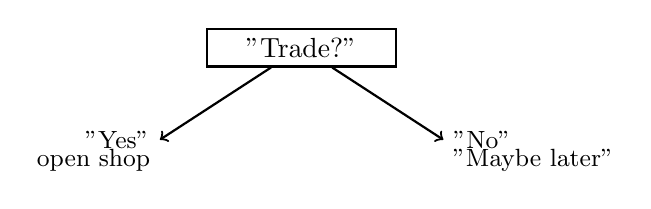
\begin{tikzpicture}[scale=0.9]

        \node[draw, thick, minimum width=2.4cm] (a) at (0,0) {"Trade?"};
        \draw[->, thick] (a) -- (-2,-1.3) node[left]{\small "Yes"};
        \draw[->, thick] (a) -- (2,-1.3) node[right]{\small "No"};
        \node[below left] at (-2,-1.3) {\small open shop};
        \node[below right] at (2,-1.3) {\small "Maybe later"};
    \end{tikzpicture}
    \end{center}
\end{frame}


\begin{frame}{String methods — transforming text}
    \large
    \begin{itemize}
        \item \texttt{.toUpperCase()} returns a NEW version
        \item It doesn't modify the original variable. String methods almost always hand back a new result.
    \end{itemize}
\end{frame}


\begin{frame}{BOSS — text, arrays, and a loop, together}
    \large
    \begin{itemize}
        \item An array of \{name, score\} objects is a real, proper data table
        \item Looping through it is exactly how every leaderboard works.
    \end{itemize}
\end{frame}

\begin{frame}{Real-World Examples}
    \large
    \begin{itemize}
        \item Any RPG's dialogue choices ("Attack" / "Defend" / "Run") branching to different outcomes, and a game's online leaderboard listing name+score pairs, are both exactly this chapter's ideas in shipped games. Minecraft villager trading menus are a real dialogue tree too
        \item Compare your held item's name against what the villager wants, branch to "trade accepted" or not.
    \end{itemize}
\end{frame}


\begin{frame}{Let Them Discover}
    \Large
    Play (or recall) a game with dialogue choices (or a Minecraft villager trade). Pick one branch and trace it: what text comparison do you think the code is making to decide which reply you see?
\end{frame}

\begin{frame}{Your Turn}
    \Large
    Open the student map, find \textbf{G9 — Strings \& Dialogue}, and work through it
    hands-on --- everything you just saw, they now do themselves.
\end{frame}

\end{document}
